\documentclass[11pt]{article}
\usepackage{geometry,marginnote} % Pour passer au format A4
\geometry{hmargin=1cm, vmargin=1cm} % 

% Page et encodage
\usepackage[T1]{fontenc} % Use 8-bit encoding that has 256 glyphs
\usepackage[english,french]{babel} % Français et anglais
\usepackage[utf8]{inputenc} 

\usepackage{lmodern,numprint}
\setlength\parindent{0pt}

% Graphiques
\usepackage{graphicx,float,grffile,units}
\usepackage{tikz,pst-eucl,pst-plot,pstricks,pst-node,pstricks-add,pst-fun,pgfplots} 

% Maths et divers
\usepackage{amsmath,amsfonts,amssymb,amsthm,verbatim}
\usepackage{multicol,enumitem,url,eurosym,gensymb,tabularx}

\DeclareUnicodeCharacter{20AC}{\euro}



% Sections
\usepackage{sectsty} % Allows customizing section commands
\allsectionsfont{\centering \normalfont\scshape}

% Tête et pied de page
\usepackage{fancyhdr} \pagestyle{fancyplain} \fancyhead{} \fancyfoot{}

\renewcommand{\headrulewidth}{0pt} % Remove header underlines
\renewcommand{\footrulewidth}{0pt} % Remove footer underlines

\newcommand{\horrule}[1]{\rule{\linewidth}{#1}} % Create horizontal rule command with 1 argument of height

\newcommand{\Pointilles}[1][3]{%
  \multido{}{#1}{\makebox[\linewidth]{\dotfill}\\[\parskip]
}}

\newtheorem{Definition}{Définition}

\usepackage{siunitx}
\sisetup{
    detect-all,
    output-decimal-marker={,},
    group-minimum-digits = 3,
    group-separator={~},
    number-unit-separator={~},
    inter-unit-product={~}
}

\setlength{\columnseprule}{1pt}

\begin{document}

\textbf{Nom, Prénom :} \hspace{8cm} \textbf{Classe :} \hspace{3cm} \textbf{Date :}\\

\vspace{-0.5cm} \begin{center}
  \textit{Pourquoi apprendre alors que l’ignorance est instantanée ?}  - \textbf{ Bill Watterson}
\end{center}

\textbf{exo1 - Calculer}

\begin{multicols}{3}
\begin{itemize}[label={$\bullet$}]
  \item $\sin(26)$ \dotfill 
  \item $\cos(26)$ \dotfill \columnbreak
  \item $\arcsin(0.44)$ \dotfill 
  \item $\arccos(0.55)$ \dotfill \columnbreak
  \  \item $\arcsin(sin(34))$ \dotfill 
  \item $\sin(34)^2 + \cos(34)^2 $ \dotfill 
\end{itemize} 
\end{multicols}

\textbf{exo2 - Nommer les cotés : hyp, adj et opp}

\begin{figure}[H]
  \centering
  
\includegraphics[width=0.6\linewidth]{4x10-trigonometrie/exo2.pdf}
\end{figure}

\textbf{exo3 - Calculer opp et adj}

\begin{figure}[H]
  \centering
  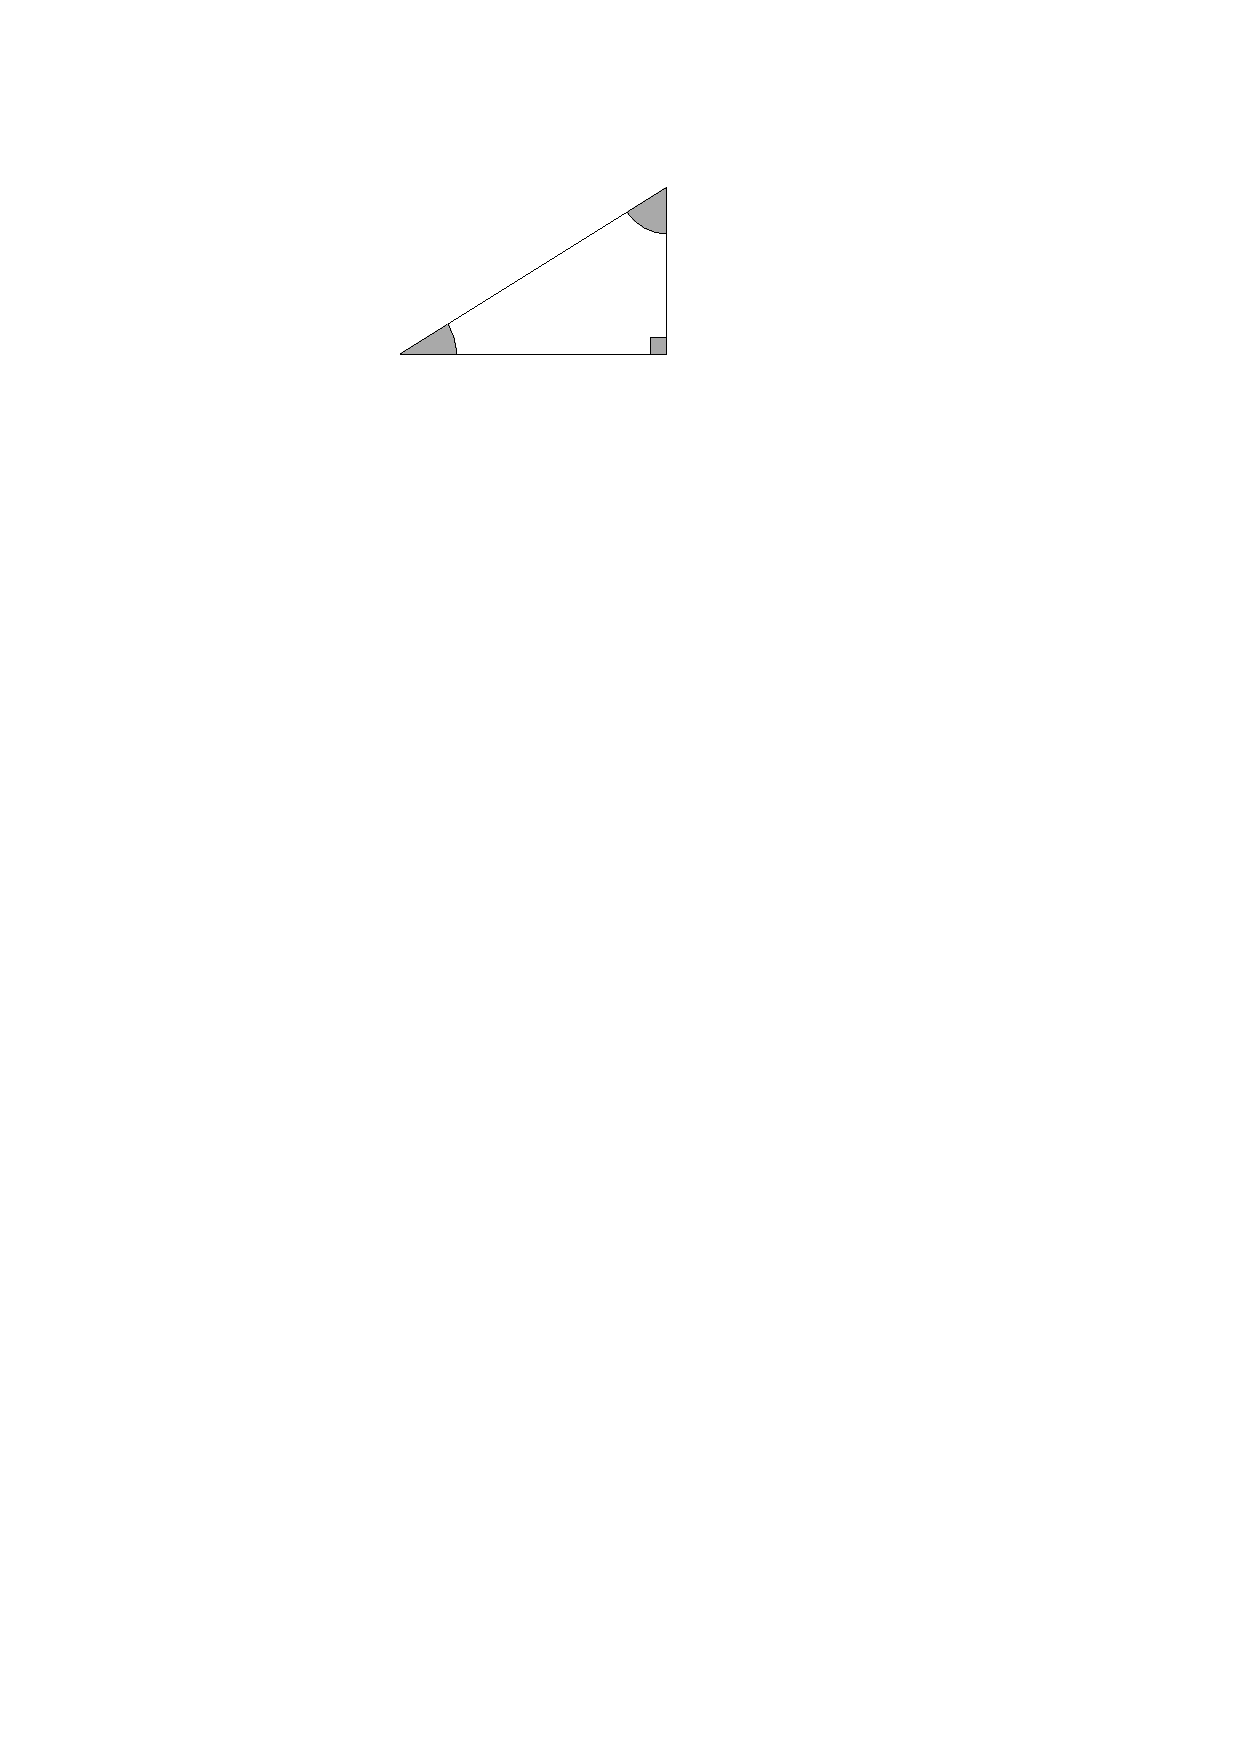
\includegraphics[width=0.6\linewidth]{4x10-trigonometrie/exo3.pdf}
\end{figure}

\Pointilles[3]

\begin{multicols}{2}

\textbf{Pb1 - Sea of Thieves}

\begin{figure}[H]
  \centering
  \includegraphics[width=0.6\linewidth]{4x10-trigonometrie/pb1a.pdf}
\end{figure}

\begin{enumerate}
  \item Dans Sea of Thieves, le bateau du joueur se déplace à la vitesse de $5,4m/s$. Il met $46s$ pour dépasser les deux points de repère. Calculer la distance parcourue ?
  \item Avec son théodolite, il mesure un angle entre les deux points de repère de 41°. Pour être dans une zone protégée qui interdit les attaques, le bateau doit être à une distance plus grande que $200m$ de la côte. Le bateau est-il en sécurité ?
\end{enumerate} \columnbreak

\Pointilles[17]

\end{multicols}

\newpage

\begin{multicols}{2}

  \textbf{Pb2 - Terre}


  \begin{figure}[H]
    \centering
    \includegraphics[width=0.5\linewidth]{4x10-trigonometrie/pb2a.pdf}
  \end{figure}
  
  Le Rayon de la Terre est $6 371 km$. 
  \begin{enumerate}
    \item Calculer la distance AF.
    \item Calculer le périmètre du \textit{parallèle} passant par F. On rappelle que $P = 2 \pi \times Rayon$.
    \item La terre fait un tour sur elle-même en une journée. \\
    Calculer la vitesse à lequelle tourne le point F en une journée.
  \end{enumerate} \columnbreak

  \textbf{Pb3 - Redline}

  \begin{figure}[H]
    \centering
    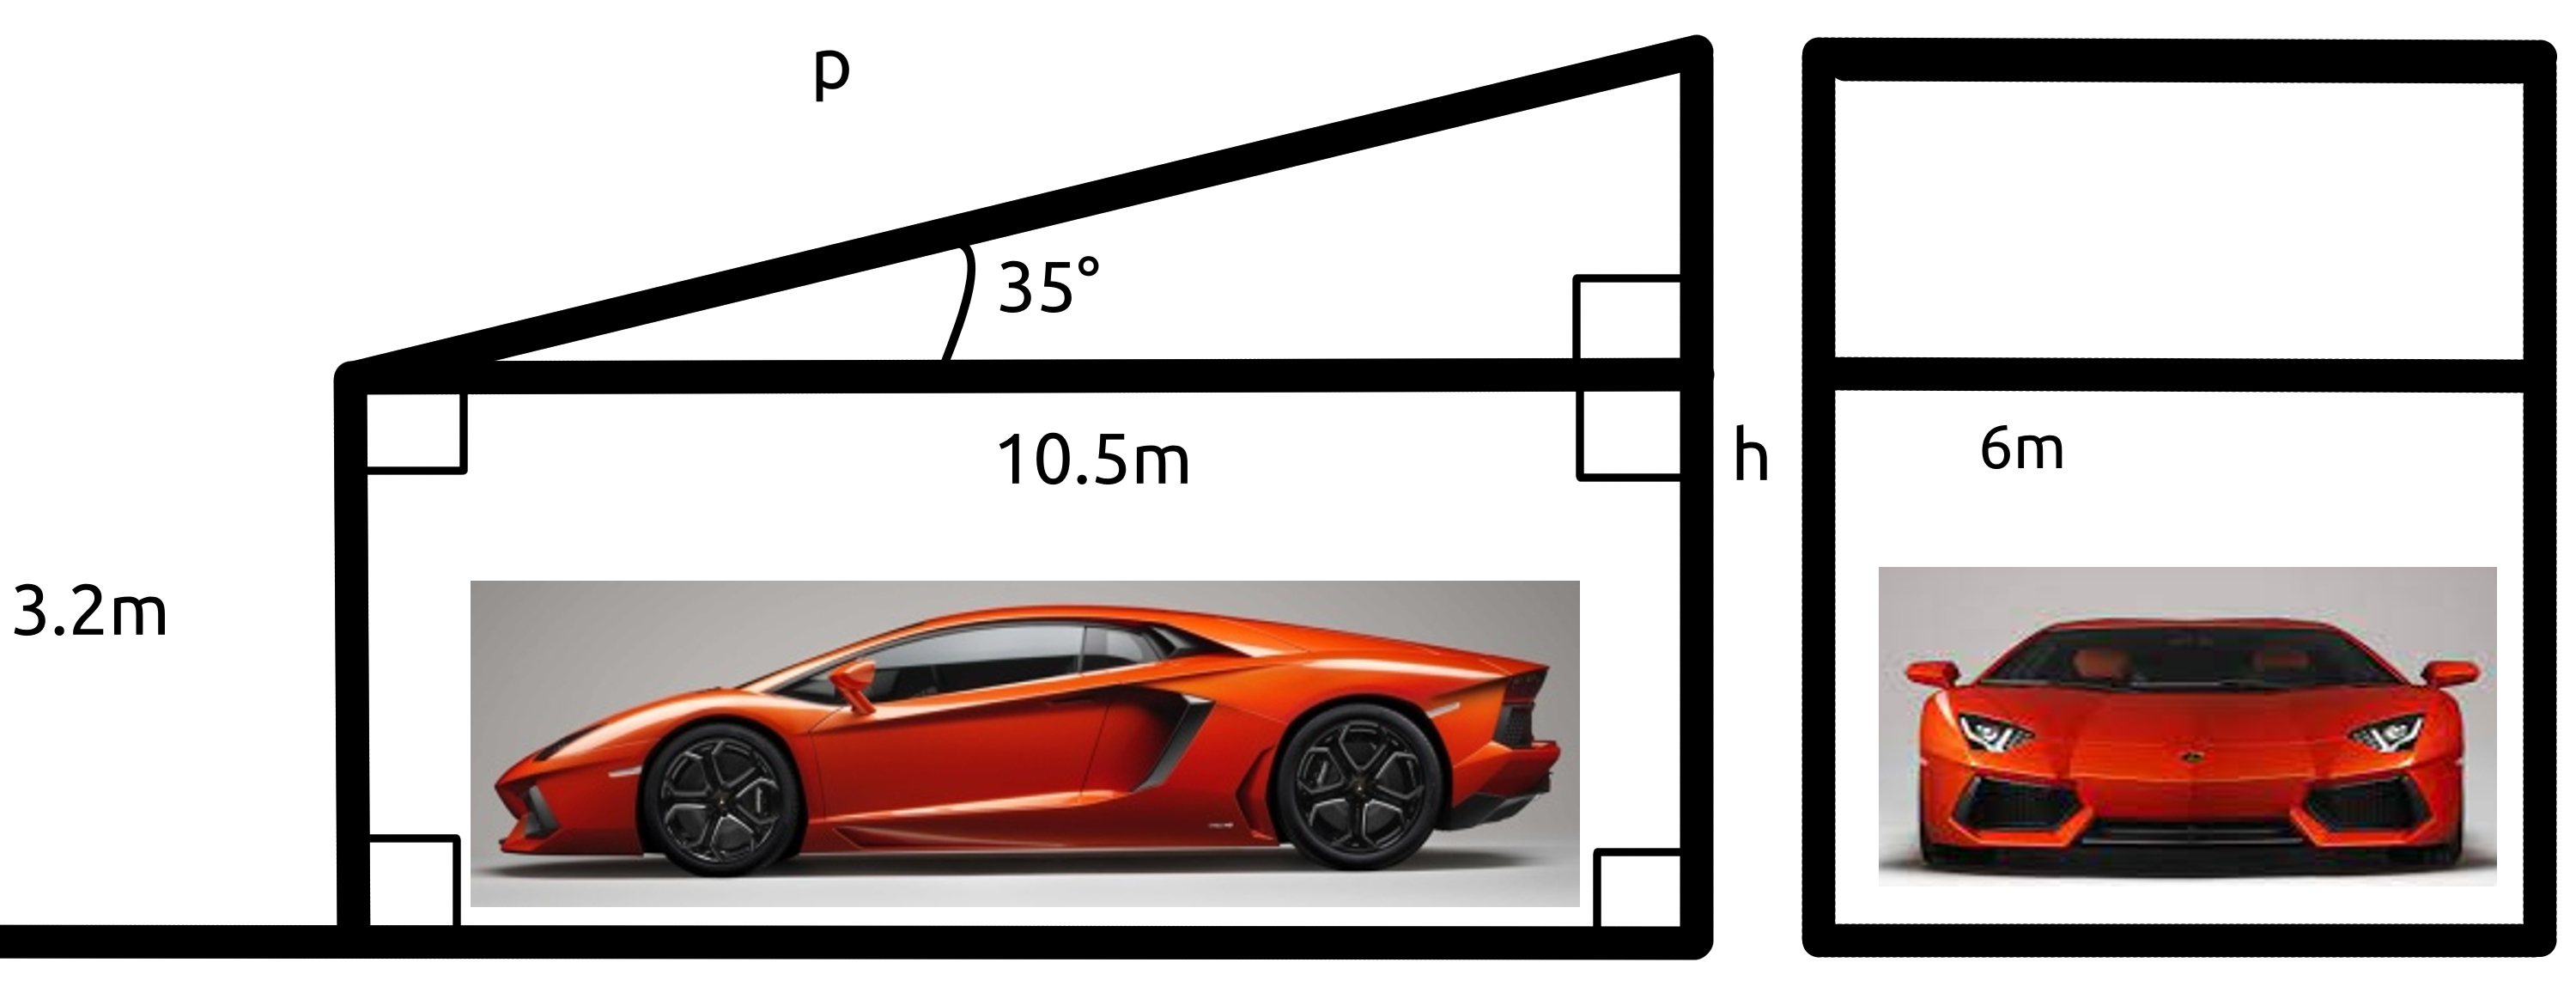
\includegraphics[width=\linewidth]{4x10-trigonometrie/pb3-1.png}
  \end{figure}
  
  \textsc{JP} doit construire un garage pour sa voiture afin de la protéger des intempéries avant de concourir sur Redline. 
  
  \begin{enumerate}
    \item Démontrer que la longueur de la poutre $p \approx 12.81m$.
    \item Calculer la hauteur $h$ à laquelle il doit fixer la poutre contre sa maison.
    \item On veut protéger le toit du garage avec des plaques d'ardoise carré de côté 50cm. Combien de plaque d'ardoise doit-on acheter ? 
  \end{enumerate} 

\end{multicols}

\Pointilles[29]

\newpage

\textbf{Nom, Prénom :} \hspace{8cm} \textbf{Classe :} \hspace{3cm} \textbf{Date :}\\

\vspace{-0.5cm} \begin{center}
  \textit{Pourquoi apprendre alors que l’ignorance est instantanée ?}  - \textbf{ Bill Watterson}
\end{center}

\textbf{exo1 - Calculer}

\begin{multicols}{3}
\begin{itemize}[label={$\bullet$}]
  \item $\sin(36)$ \dotfill 
  \item $\cos(36)$ \dotfill \columnbreak
  \item $\arcsin(0.24)$ \dotfill 
  \item $\arccos(0.75)$ \dotfill \columnbreak
  \  \item $\arcsin(sin(74))$ \dotfill 
  \item $\sin(28)^2 + \cos(28)^2 $ \dotfill 
\end{itemize} 
\end{multicols}

\textbf{exo2 - Nommer les cotés : hyp, adj et opp}

\begin{figure}[H]
  \centering
  
\includegraphics[width=0.6\linewidth]{4x10-trigonometrie/exo2.pdf}
\end{figure}

\textbf{exo3 - Calculer opp et adj}

\begin{figure}[H]
  \centering
  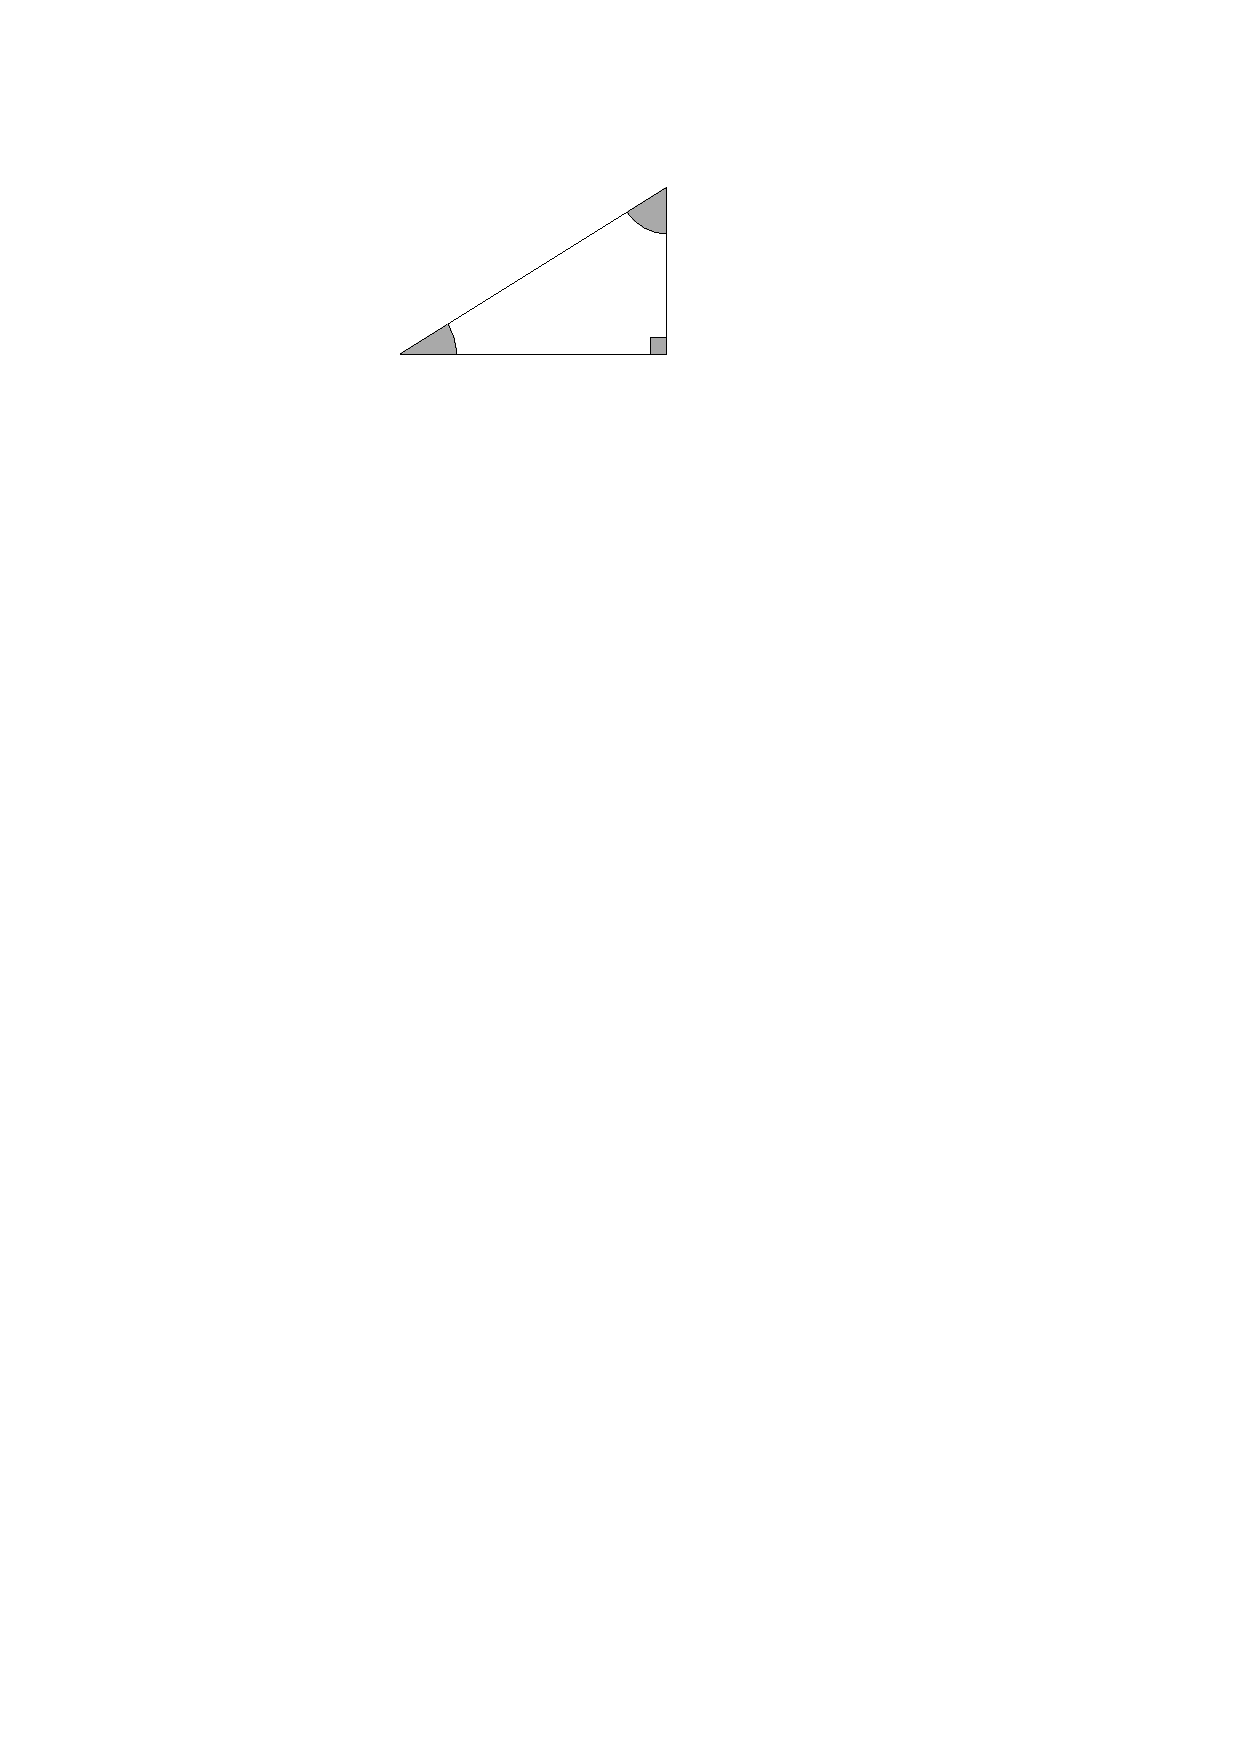
\includegraphics[width=0.6\linewidth]{4x10-trigonometrie/exo3.pdf}
\end{figure}

\Pointilles[3]

\begin{multicols}{2}

\textbf{Pb1 - Sea of Thieves}

\begin{figure}[H]
  \centering
  \includegraphics[width=0.6\linewidth]{4x10-trigonometrie/pb1a.pdf}
\end{figure}

\begin{enumerate}
  \item Dans Sea of Thieves, le bateau du joueur se déplace à la vitesse de $5,1m/s$. Il met $54s$ pour dépasser les deux points de repère. Calculer la distance parcourue ?
  \item Avec son théodolite, il mesure un angle entre les deux points de repère de 41°. Pour être dans une zone protégée qui interdit les attaques, le bateau doit être à une distance plus grande que $250m$ de la côte. Le bateau est-il en sécurité ?
\end{enumerate} \columnbreak

\Pointilles[17]

\end{multicols}

\newpage

\begin{multicols}{2}

  \textbf{Pb2 - Terre}


  \begin{figure}[H]
    \centering
    \includegraphics[width=0.5\linewidth]{4x10-trigonometrie/pb2a.pdf}
  \end{figure}
  
  Le Rayon de la Terre est $6 371 km$. 
  \begin{enumerate}
    \item Calculer la distance AF.
    \item Calculer le périmètre du \textit{parallèle} passant par F. On rappelle que $P = 2 \pi \times Rayon$.
    \item La terre fait un tour sur elle-même en une journée. \\
    Calculer la vitesse à lequelle tourne le point F en une journée.
  \end{enumerate} \columnbreak

  \textbf{Pb3 - Redline}

  \begin{figure}[H]
    \centering
    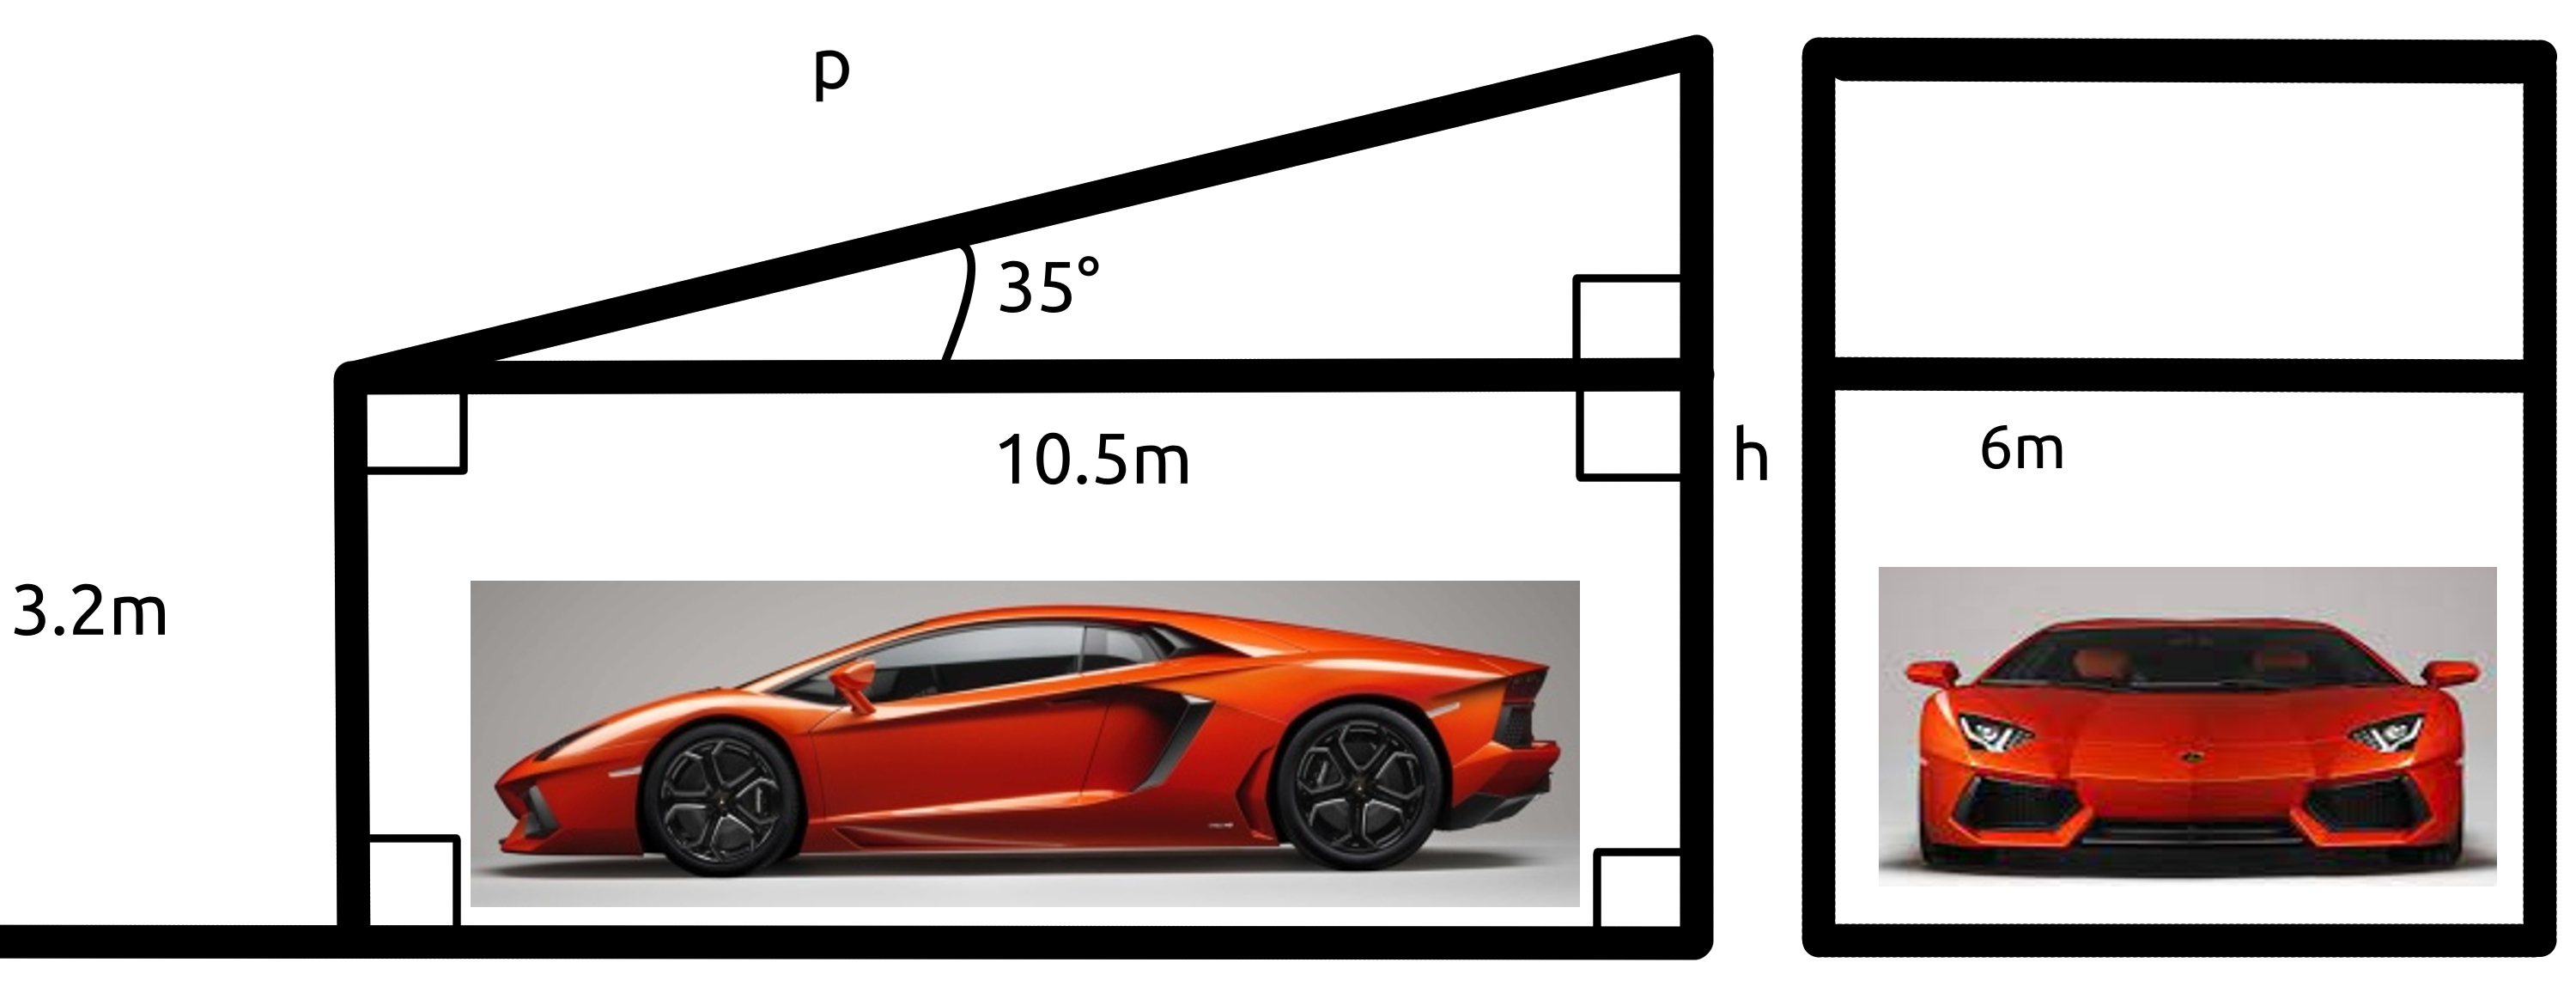
\includegraphics[width=\linewidth]{4x10-trigonometrie/pb3-1.png}
  \end{figure}
  
  \textsc{JP} doit construire un garage pour sa voiture afin de la protéger des intempéries avant de concourir sur Redline. 
  
  \begin{enumerate}
    \item Démontrer que la longueur de la poutre $p \approx 12.81m$.
    \item Calculer la hauteur $h$ à laquelle il doit fixer la poutre contre sa maison.
    \item On veut protéger le toit du garage avec des plaques d'ardoise carré de côté 50cm. Combien de plaque d'ardoise doit-on acheter ? 
  \end{enumerate} 

\end{multicols}

\Pointilles[29]


\end{document}
